\documentclass[11pt,a4paper]{article}

\usepackage[slovene]{babel}
\usepackage{color}
\usepackage{graphicx}
\usepackage{verbatim}
\usepackage{amsmath}
\usepackage{tikz}
\usepackage{esvect}
\usepackage{float}
\usepackage{xcolor}
\usepackage{listings}
\usepackage{xparse}

\usepackage[backend=bibtex]{biblatex}

% code styling
\lstset{language=Python,keywordstyle={\bfseries \color{blue}}}
\NewDocumentCommand{\codeword}{v}{%
	\texttt{\textcolor{blue}{#1}}%
}

\addbibresource{viri.bib}

\begin{document}

\title{Povratek kapsule v ozra\v cje}
\author{\v Ziga Pata\v cko Koderman}
\date{\today}

\clearpage\maketitle
\thispagestyle{empty}
\pagebreak

\tableofcontents
\pagebreak

\section{Uvod}

Povratek kapsule iz vesolja neki neki neki

To poro\v cilo posku\v sa oceniti kot, pod katerim moramo pri... jebes, nemorem zdele tega napisat.

\pagebreak

\section{Fizikalno ozadje}
\subsection{Sile}

Za opis gibanja kapsule pri ponovnem vstopu v atmosfero bomo upo\v stevali silo gravitacije planeta na kapsulo $F_g$, silo zra\v cnega upora $F_u$ ter silo vzgona $F_v$. Za te velja:


\begin{equation}
F_g(h) = m g(h)
\end{equation}

\begin{equation}
F_u(v, h) = k_{u}\rho (h) v^2
\end{equation}

\begin{equation}
F_v(h) = V \rho(h)
\end{equation} \\
Kjer sta gravitacijski pospe\v sek $g(h)$ ter koeficient upora $k_u$:

\begin{equation}
g(h) = g_0 (\frac{r}{r+h})^2
\end{equation}

\begin{equation}
k_u = \frac{Sc_u}{2}
\end{equation}
kjer $c_u$ predstavlja koeficient upora oblike kapsule. \\ \\

Gostoto zraka v odvisnosti od vi\v sine pa izpeljemo:
$$ \frac{dp}{dh} = -\rho g $$
$$ \rho = \frac{n M }{V} $$
Z uporabo plinskega zakona za idealni plin $ pV = nRT $ zamenjamo $n$:
$$ \rho = \frac{pM}{RT} $$
In vstavimo v prvo ena\v cbo:
$$ \frac{1}{p} dp = - \frac{Mg}{RT} dh$$
Po integraciji ostane:
$$ p = p_0 e ^{-\frac{h}{H}} $$
kjer je $H = \frac{RT}{Mg}$ vi\v sina, pri kateri se tlak zmanj\v sa za $\frac{1}{e}$. Ker pa sta tlak in gostota zraka premo sorazmerna, lahko uporabimo isti $H$ tudi za gostoto. Sledi:
\begin{equation}
\rho(h) = \rho_0 e^{-\frac{h}{H}}
\end{equation}

\subsection{Ena\v cbe gibanja in koordinatni sistem}

Za la\v zje obravnavanje ena\v cb in numeri\v cno integriranje bomo uporabili koordinatni sistem, ki ima izhodi\v sce v sredi\v s\v cu plovila, njegova $x$ os pa je pravokotna na zveznico med sredi\v s\v cem planeta ter kapsulo.

\vspace{0.5cm}

\begin{figure}[H]
	\centering
	\begin{tikzpicture}[scale=.95]
	\draw (0, 0) circle (4);
	\draw[dashed] (0, 0) circle (4.2);
	\draw[->, rotate=-30] (0,0) -- (0, 4) node[below] {$r$}; % r
	\draw[->, rotate=-30] (0,4) -- node[above] {$h$}  (0, 5); % h
	\draw[->, rotate=-30] (0,5) -- (2, 5) node[below] {$x$}; % x
	\draw[->, rotate=-30] (0,5) -- (0, 7) node[above] {$y$}; % y
	\draw[->, rotate=-30] (0,5) -- (1.8, 6.25) node[above]{$\vv{v}$}; % v
	\draw [->, rotate=-30](0,5) -- (1.2,5) arc (0:35:1.2cm) node[below left]{$-\gamma$};
	\draw[dashed] (0,0) -- (0, 7); % x fixed
	\draw [dashed, ->, rotate=90] (0,0) -- (2,0) node[below right]{$\phi$} arc (0:-30:2cm);
	\end{tikzpicture}
	\caption{Relativni koordinatni sistem kapsule glede na planet}
	\label{fig:sp2d}
\end{figure}

Glede na novi kordinatni sistem zapi\v semo diferencialne ena\v cbe gibanja. Hitrost v horizontalni smeri je
\begin{equation}
	\dot{x} = v * cos(\gamma),
\end{equation}
v vertikalni pa
\begin{equation}
	\dot{h} = v * sin(\gamma).
\end{equation}
Absolutni pospe\v sek sestavljata vertikalna komponenta $g$ ter sila upora:
\begin{equation}
	\dot{v} = g*sin(\gamma) - \rho(h) v^2 k_u.
\end{equation}
Odvod kota $\gamma$ pa izpeljemo. V pozitivno smer nanj vpljiva gravitacijski pospe\v sek z velikostjo $g\frac{cos(\gamma)}{v}$. V negativno smer na kot $\gamma$ vpljiva premik zaradi vztrajnostnega momenta. Velikost tega \v clena je odvisna od krivinskega radija planeta in se glasi $ -v \frac{cos(\gamma)}{r}$.\\ \\
Za upo\v stevanje sile vzgona pa potrebujemo manjka !!!\textsl{}! \\\\
Sprememba kota $\gamma$ se torej glasi
\begin{equation}
	\dot{\gamma} = g\frac{cos(\gamma)}{v}  - v \frac{cos(\gamma)}{r} - \alpha v k*rho(h)
\end{equation}
kjer je $\alpha$ razmerje med silo vzgona in silo upora kapsule.\\

Te \v stiri ena\v cbe zadostujejo za simulacijo leta kapsule. Za la\v zje risanje sheme  leta kapsule skozi atmosfero pa bomo spremljali \v se vrednost kota $\phi$ v odvisnosti od \v casa.
\begin{equation}
	\dot{\phi} = v \frac{cos(b)}{r+h}
\end{equation}
\newpage

\section{Simulacija}
Spremenljivke v simulaciji so torej $\{x, h, v, \beta, \phi \}$, potek gibanja kapsule pa je odvisen od njihovih za\v cetnih vrednosti $x_0 = 0$, $h_0$, $v_0$ ter $\beta_0 = 0$. Nas pa posebaj zanima za\v cetni kot $\phi_0$, ki nam pove, s kak\v snim za\v cetnim kotom se zaletimo v atmosfero.

Od tega je odvisno s kak\v snim pospe\v skom nas bo atmosfera zaustavljala in ali se bomo morebiti odbili nazaj v vesolje. Kriteriji za uspe\v sen povratek bodo:
\begin{itemize}
	\item najve\v cji pospe\v sek bo manj\v si od $10 g$,
	\item na tleh bo kapsula pristala v manj kot $30$ min ($1800$ s).
\end{itemize}
Posebej pa nas zanimajo koti, pri katerih sta maksimalna mo\v c in pospe\v sek najmanjsa. \\

Za simulacijo gibanja kapsule bomo uporabili funkcijo \codeword{odeint()} iz Pythonove knji\v znjice scypy. Tej podamo funkcijo, ki ra\v cuna odvode \v zeljenih spremenljivk v danih to\v ckah. V na\v sem primeru poenostavljena razli\v cica te funkcije izgleda takole: \\
\begin{lstlisting}
def movement(parametres, t, sim):
	x, h, v, b, phi = parametres

	dxdt = v * np.cos(b)
	dhdt = -v * np.sin(b)
	dvdt = sim.g(h) * np.sin(b) - sim.rho(h) *
			sim.capsule['k'] * v ** 2
			
	dbdt = sim.g(h) * np.cos(b) / v - v *
			np.cos(b) / sim.planet['r']
			
	if not sim.ignore_buoyancy:
		dbdt -= sim.rho(h) * v *
			sim.capsule['k'] *
			sim.capsule['l2d']
			
	dphidt = v * np.cos(b) /
			(sim.planet['r'] + h)

	return [dxdt, dhdt, dvdt, dbdt, dphidt]
\end{lstlisting}
\clearpage
%\vspace{0.5cm}

Da najdemo optimalen vstopni kot, bomo predpostavili, da vstopa kapsule ne moremo kontrolirati natan\v cneje kot na $0.01^\circ $. Tako se lahko s korakom $0.01^\circ $ sprehodimo med kotoma $0^\circ$ in $15^\circ$ (ki je zagotovo prevelik za povratek kapsule iz vesolja). \\

\section{Primer povratka Apollo kapsule}
Da preverimo pravilnost na\v se simulacije, bomo za za\v cetno hitrost in druge podatke o kapsuli vzeli kar pribli\v zne vrednosti za kapsule poletov Apollo:

\begin{table}[H]
	\centering
	\caption{Lastnosti Apollo kapsule \cite{lift-and-drag-of-apollo-command-module} \cite{command-module-overview} \cite{entry-aerodynamics} }
	\vspace{0.3cm}
	\def\arraystretch{1.5}
	\begin{tabular}{l|r}
		$h_0$ & $100 \; km$ \\
		$v_0$ & $11000 \; \frac{m}{s}$ \\
		$k_{upora}$ & $1.2$ \\
		$S$ & $12 \; m^2$ \\
		$m$ & $5357 \; kg $\\
		$\alpha$ & $0.225$ \\
		$v_{padalo}$ & $111 \; \frac{m}{s}$
	\end{tabular}
	\def\arraystretch{1}
\end{table}
\vspace{0.4cm}
Potrebijemo tudi podatke o Zemlji in njeni atmosferi:
\begin{table}[H]
	\centering
	\caption{Lastnosti Zemlje \cite{earths-atmosphere}}
	\vspace{0.3cm}
	\def\arraystretch{1.5}
	\begin{tabular}{l|r}
		$g_0$ & $9.81 \; \frac{m}{s^2}$ \\
		$r$ & $3396.2 \; km$ \\
		$T$ & $236.7 K$ \\
		$M$ & $28.95$ \\
		$\rho_0$ & $1.225 \frac{kg}{m^3} $
	\end{tabular}
	\def\arraystretch{1}
\end{table}

\clearpage

\subsection{Rezultati}
tuki dam notr vs tabeli (kot, max a, max p, visina odprja padala, bool a je biu uspesn pristanek) za z vzgonom in brez. pol preberem vn keri koti so primerni, pokomentiram vse te v povezavi z pravimi koti apola in tega da uresnici oni z aerodinamiko spreminjajo l/d da bol tocno pristajajo. pokomentiram tut zakaj je vzgon zjebe use skupi (nevem?).

\clearpage
\section{Zaklju\v cek}
zabauno, kako bi izbolsou tole simulacijo (jebiga, nevem), pa da bi probu se na drugih planetih
%\vspace{1cm}

%\begin{figure}
%  \begin{center}
%  	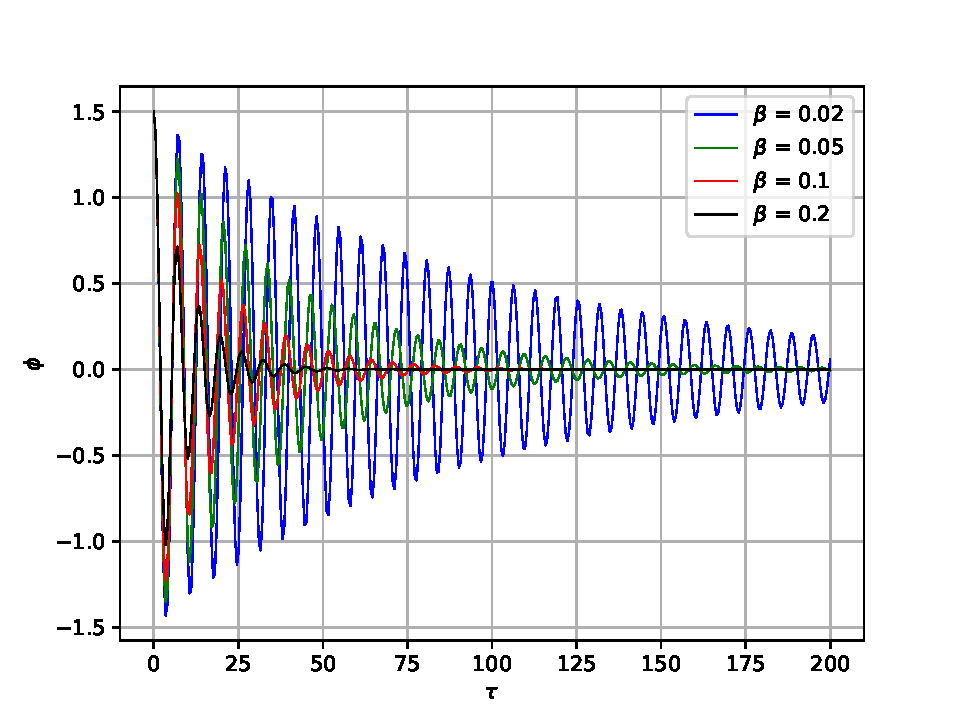
\includegraphics[width=12cm]{graf1.pdf}
%    \caption{Graf $\phi$ v odvisnosti od $\tau$}
%  \end{center}
%\end{figure}
%
%\begin{figure}
%  \begin{center}
%  	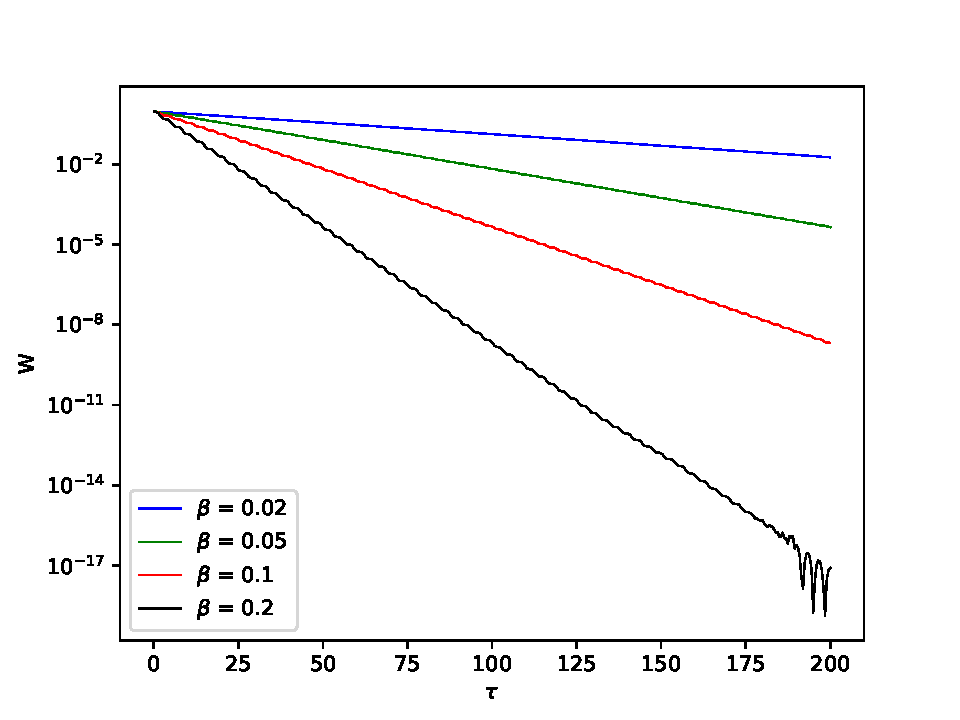
\includegraphics[width=12cm]{graf2.pdf}
%    \caption{Graf energije v odvisnosti od $\tau$ v logaritmski skali}
%  \end{center}
%\end{figure}

\vspace{2cm}


\clearpage
\section{Literatura}
\printbibliography[heading=none]
\end{document}
